%% Requires compilation with XeLaTeX or LuaLaTeX
\documentclass[compress,10pt,xcolor={table,dvipsnames},t]{beamer}
\usetheme{diapo}
\usepackage{amsmath}
\usepackage{amssymb}
\usepackage{xcolor}
\usepackage[bottom]{footmisc}
\usepackage{multirow}
\usepackage{setspace}
\usepackage{caption}
\usepackage{array,multirow,makecell}
\usepackage{pifont}
\usepackage{tikz}
\usepackage{paralist}
\usepackage{appendixnumberbeamer}
\usepackage[style=numeric,sorting=nyt,doi=false,url=false,maxbibnames=99,date=year]{biblatex}
\usepackage{etoolbox}
% box colorée dans équation
\usepackage[most]{tcolorbox}
\usepackage{tikz}
\usepackage{soul}
% pour l'indicatrice
\usepackage{dsfont}
\usepackage{cancel}

%%% configurer bibliographie

% Charger votre fichier de bibliographie
\addbibresource{biblio.bib}

% Définir les champs à ne pas afficher dans la bibliographie
\AtEveryBibitem{
	\clearlist{language}
	\clearfield{note}
	\clearfield{edition}
	\clearfield{series}
	\clearfield{url}
	\clearfield{urldate}
	\clearfield{pagetotal}
	\clearfield{pages}
	\clearfield{issn}
	\clearfield{doi}
	\clearfield{url}
	\clearfield{eprint}
}

% Définir le style des citations
\DeclareFieldFormat{title}{\textit{#1}}
\DeclareFieldFormat[article]{title}{#1}
\DeclareNameAlias{sortname}{last-first}
\DeclareFieldFormat{author}{#1.}

% Choisir les informations à afficher dans la bibliographie
\renewbibmacro{in:}{}
\renewbibmacro*{journal+issuetitle}{%
	\ifentrytype{article}{
		\usebibmacro{journal}
	}{%
		\printfield{title}%
	}%
}

\renewbibmacro*{date}{%
	\ifentrytype{misc}{%
		\printtext{\printdate}%
	}{%
		\printdate
	}%
}
%% fin configuration biblio

\setcellgapes{1pt}
\setlength{\parindent}{0pt}
\makegapedcells
\newcolumntype{R}[1]{>{\raggedleft\arraybackslash }b{#1}}
\newcolumntype{L}[1]{>{\raggedright\arraybackslash }b{#1}}
\newcolumntype{C}[1]{>{\centering\arraybackslash }b{#1}}
\renewcommand*{\bibfont}{\scriptsize}
\useoutertheme[subsection=false]{miniframes}
\makeatletter
%\patchcmd{\slideentry}{\advance\beamer@xpos by1\relax}{}{}{}
\def\beamer@subsectionentry#1#2#3#4#5{\advance\beamer@xpos by1\relax}%
\makeatother
\setbeamercolor*{mini frame}{fg=bulles,bg=bulles}
\hypersetup{
	colorlinks=true,
	urlcolor=blue,
	citecolor=blue,
	linkcolor=title,
}

\title[PhiFEM]{Mesh-based methods and physically informed learning}
\subtitle{Macaron/Tonus retreat presentation}
\authors[LECOURTIER Frédérique]
\supervisors[DUPREZ Michel, FRANCK Emmanuel, LLERAS Vanessa]
\date{February 6-7, 2024}

\allowbreak

% u_chapeau (chapeau en couleur)
\usepackage{accents}
\newcommand{\uchapeau}[1]{\accentset{\textcolor{red}{\wedge}}{#1}}
\newcommand{\refappendix}[1]{\tikz[baseline=(char.base)]{\node[framednumber] (char) {\hyperlink{#1}{\small \textcolor{white}{Appendix \ref*{#1}}}};}}

\definecolor{appendix}{RGB}{180, 189, 138}
\tikzset{
	framednumber/.style={
		draw=appendix,% Couleur de la bordure
		fill=appendix, % Couleur de fond
		rounded corners, % Coins arrondis
		inner sep=2pt,  % Espace intérieur
	}
}

% numérotation et label des appendix
\newcounter{appendixframenumber}
\setcounter{appendixframenumber}{1}

\makeatletter
\newcommand{\labelappendixframe}[1]{%
	\protected@write\@auxout{}{%
		\string\newlabel{#1}{{\theappendixframenumber}{\thepage}}%
	}%
	\hypertarget{#1}{}
}	
\makeatother

%\newenvironment{appendixframe}[2][]{%
%	\begin{frame}[#1]{\appendixname~\theappendixframenumber~: #2}%
%	}{%
%	\end{frame}
%	\addtocounter{appendixframenumber}{1}
%}

% barre en couleur terme dans équation
\newcommand\Ccancel[2][black]{\renewcommand\CancelColor{\color{#1}}\cancel{#2}}

\begin{document}
	\nocite{*}
	
	\renewcommand{\inserttotalframenumber}{\pageref{lastslide}}
	
	{\setbeamertemplate{footline}{} 
		\begin{frame}
			\maketitle
		\end{frame}
	}
	\addtocounter{framenumber}{-1} 
	
	\AtBeginSection[]{
		{\setbeamertemplate{footline}{}
			\begin{frame}
				\vfill
				\centering
				\begin{beamercolorbox}[sep=5pt,shadow=true,rounded=true]{subtitle}
					\usebeamerfont{title}\insertsectionhead\par%
				\end{beamercolorbox}
				%\tableofcontents[sectionstyle=hide,subsectionstyle=show]
				
				%subsectionstyle=⟨style for current subsection⟩/⟨style for other subsections in current section⟩/⟨style for subsections in other sections⟩
				\tableofcontents[sectionstyle=hide,subsectionstyle=show/show/hide]
				\vfill
			\end{frame}
		}
		\addtocounter{framenumber}{-1} 
	}
	
	\AtBeginSubsection[]{
		{\setbeamertemplate{footline}{}
			\begin{frame}
				\vfill
				\centering
				\begin{beamercolorbox}[sep=5pt,shadow=true,rounded=true]{subtitle}
					\usebeamerfont{title}\insertsectionhead\par%
				\end{beamercolorbox}
				\tableofcontents[sectionstyle=hide,subsectionstyle=show/shaded/hide]
				\vfill
			\end{frame}
		}
		\addtocounter{framenumber}{-1} 
	}
	
	\section{Introduction}
	\begin{frame}{Scientific context}
    \textbf{Context :} Create real-time digital twins of an organ (such as the liver).

    \textbf{$\phi$-FEM Method :} New fictitious domain finite element method.

    \begin{enumerate}[\ding{217}]
        \item domain given by a level-set function $\Rightarrow$ don't require a mesh fitting the boundary 
        \item allow to work on complex geometries 
        \item ensure geometric quality 
        % \item Cartesian grid adapted for neural networks
    \end{enumerate}
    
    \begin{center}
        \pgfimage[width=0.65\linewidth]{images/intro/context_geometry.png}
    \end{center}	

    \textit{Practical case:} Real-time simulation, shape optimization...
\end{frame}

\begin{frame}{Objective}
    \textbf{Current Objective :} Develop hybrid finite element / neural network methods.

	\begin{center}
		\begin{tcolorbox}[
			colback=white, % Couleur de fond de la boîte
			colframe=other, % Couleur du cadre de la boîte
			arc=2mm, % Rayon de l'arrondi des coins
			boxrule=0.5pt, % Épaisseur du cadre de la boîte
			breakable, enhanced jigsaw,
			width=0.8\linewidth
			]
			
			\textbf{OFFLINE :}
			
			\begin{figure}[htb]
				\centering
				\resizebox{\textwidth}{!}{%
					\begin{tikzpicture}
						\node at (0,0.8) {Several Geometries};
						\node[draw=none, inner sep=0pt] at (0,0) {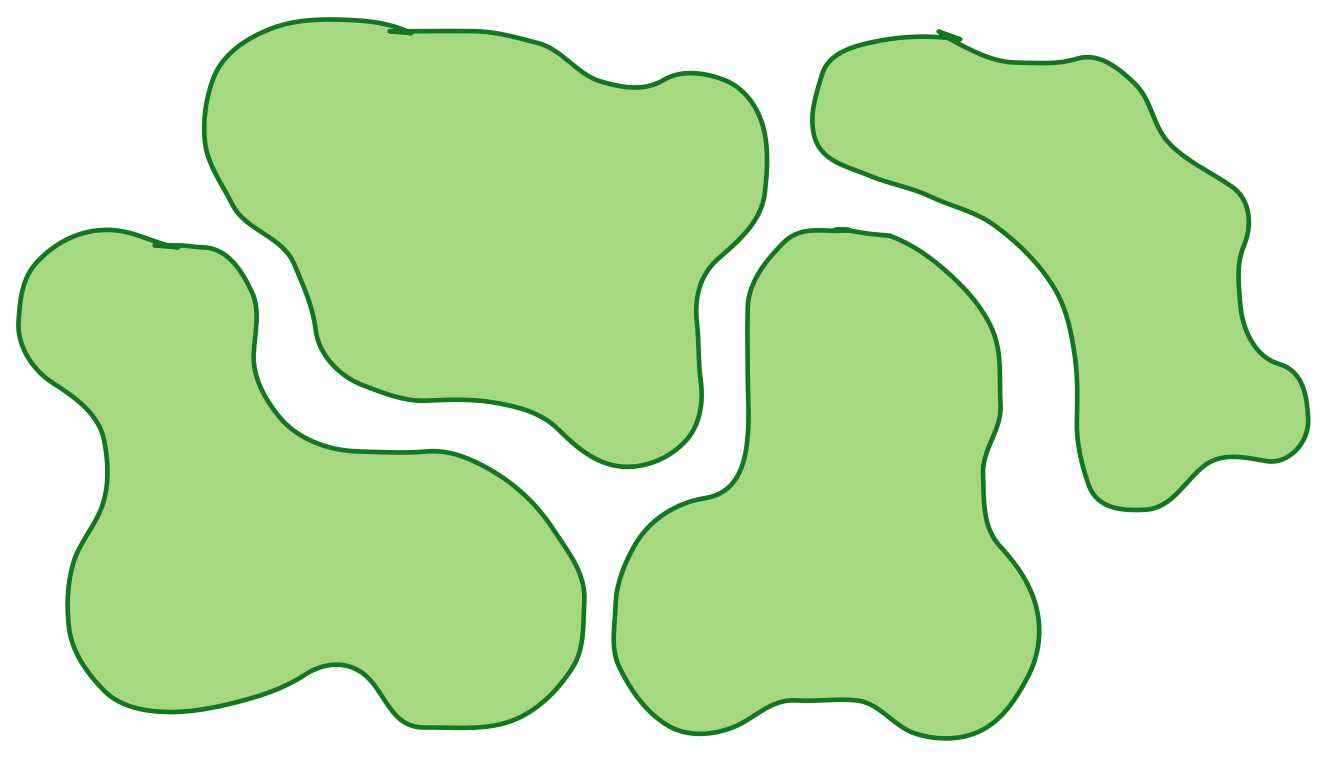
\includegraphics[width=2cm]{images/intro/objective_geom.png}};
						\node[title,font=\Large] at (1.6,0.1) {+};
						\node at (3.5,0.8) {Several Functions};
						\node[draw=none, inner sep=0pt] at (3.5,0) {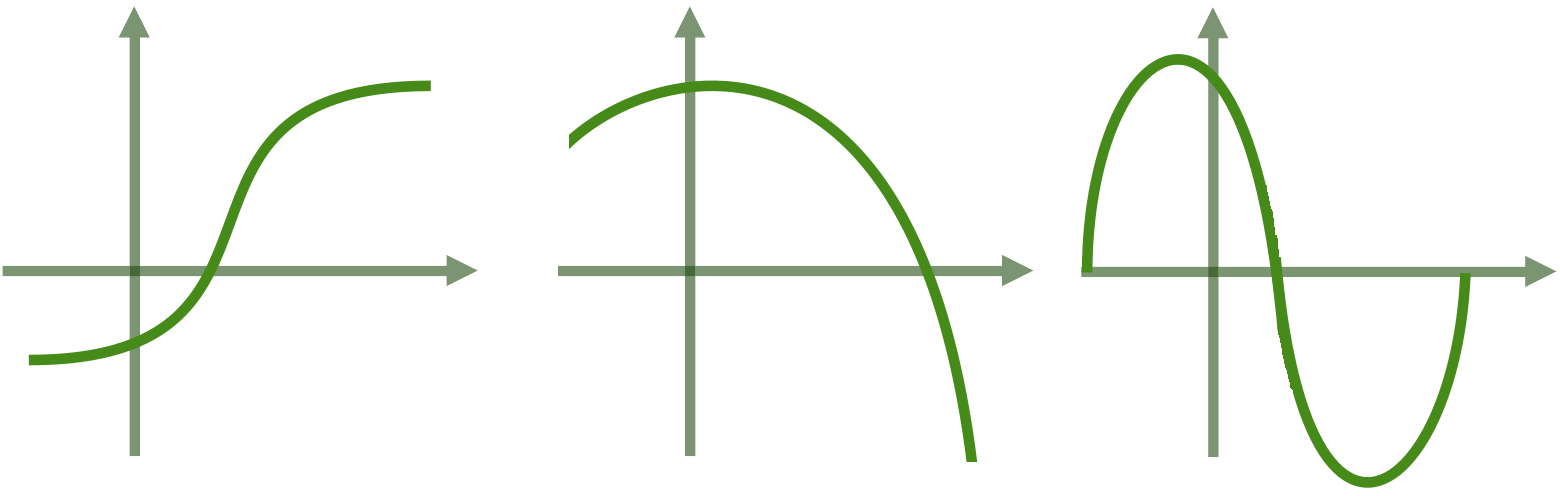
\includegraphics[width=3cm]{images/intro/objective_fct.png}};
						
						% Ajouter une flèche entre les deux rectangles
						\draw[->, title, line width=1.5pt] (5.5,0.1) -- (6.5,0.1);
						%		
						\node at (8,0.8) {Train a PINNs};
						\node[draw=none, inner sep=0pt] at (8,-0.1) {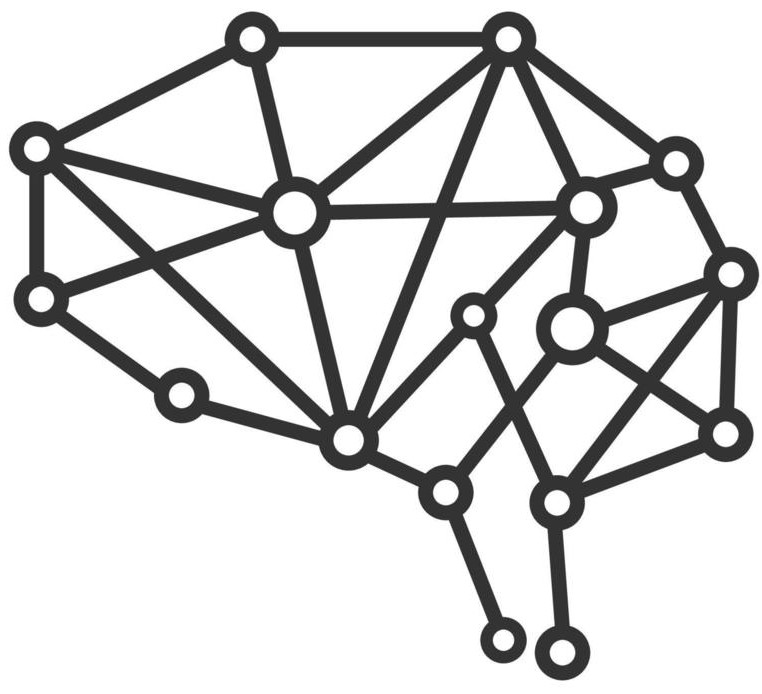
\includegraphics[width=1.5cm]{images/intro/objective_pinns.jpg}};				
					\end{tikzpicture}
				}%
			\end{figure}
			
			\textbf{ONLINE :}
			
			\vspace{-25pt}
			
			\begin{figure}[htb]
				\centering
				\resizebox{\textwidth}{!}{%
					\begin{tikzpicture}
						\node at (0,0.8) {1 Geometry - 1 Function};
						\node[draw=none, inner sep=0pt] at (0,0) {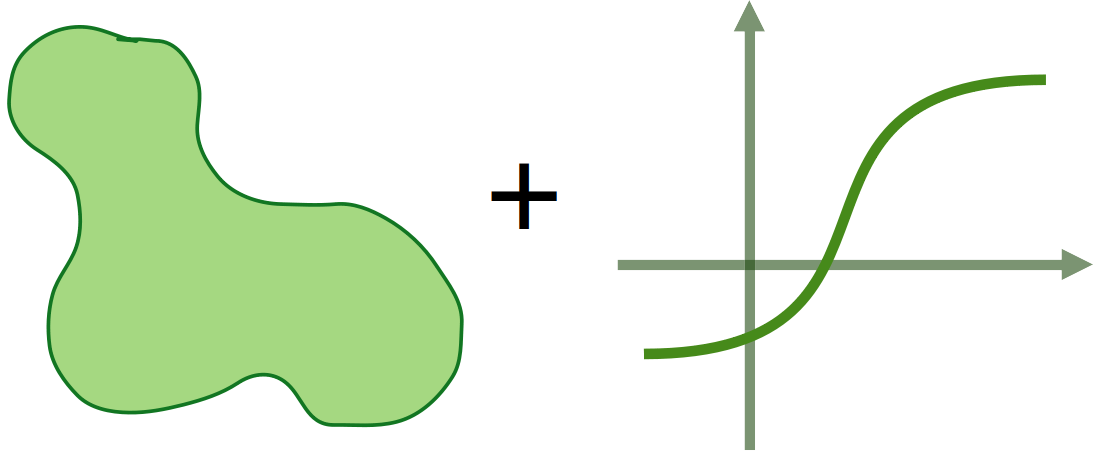
\includegraphics[width=2cm]{images/intro/objective_onegeom_onefct.png}};
						%		\node[title,font=\Large] at (1.6,0.1) {+};
						%		\node at (3.5,0.8) {Several Functions};
						%		\node[draw=none, inner sep=0pt] at (3.5,0) {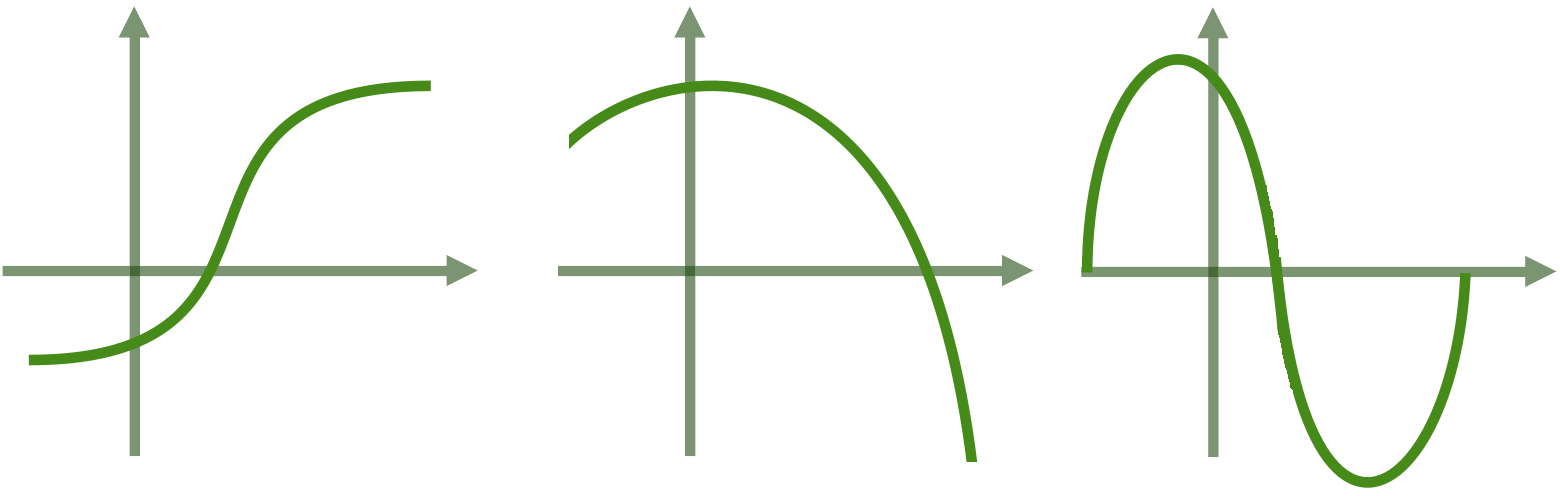
\includegraphics[width=3cm]{images/intro/objective_fct.png}};
						
						\draw[->, title, line width=1.5pt] (2,0.1) -- (3,0.1);
						
						\node[align=center] at (4,1) {Get PINNs \\ prediction};
						\node[draw=none, inner sep=0pt] at (4,-0.1) {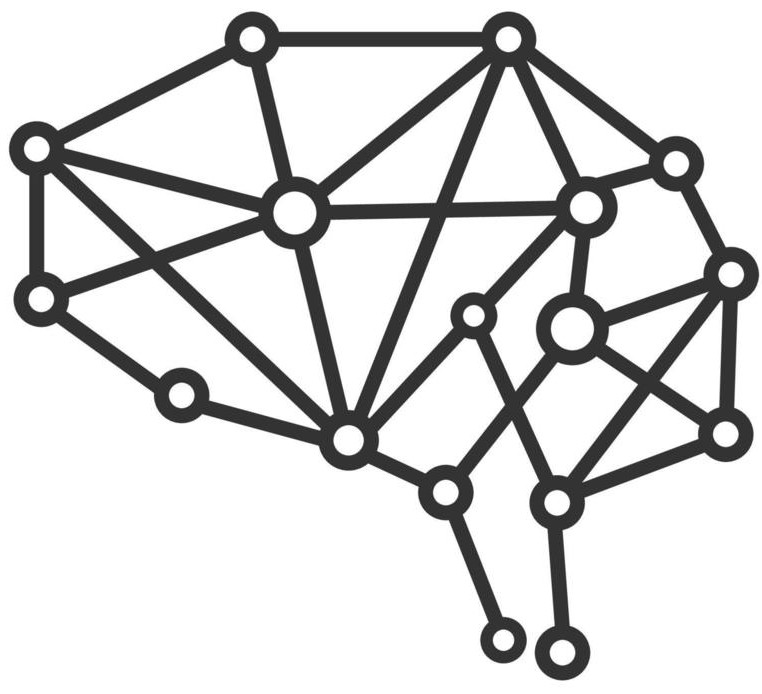
\includegraphics[width=1.5cm]{images/intro/objective_pinns.jpg}};
						
						% Ajouter une flèche entre les deux rectangles
						\draw[->, title, line width=1.5pt] (5.5,0.1) -- (6.5,0.1);
						%		
						\node[align=center] at (8,1) {Correct prediction \\ with $\phi$-FEM};
						\node[draw=none, inner sep=0pt] at (8,-0.1) {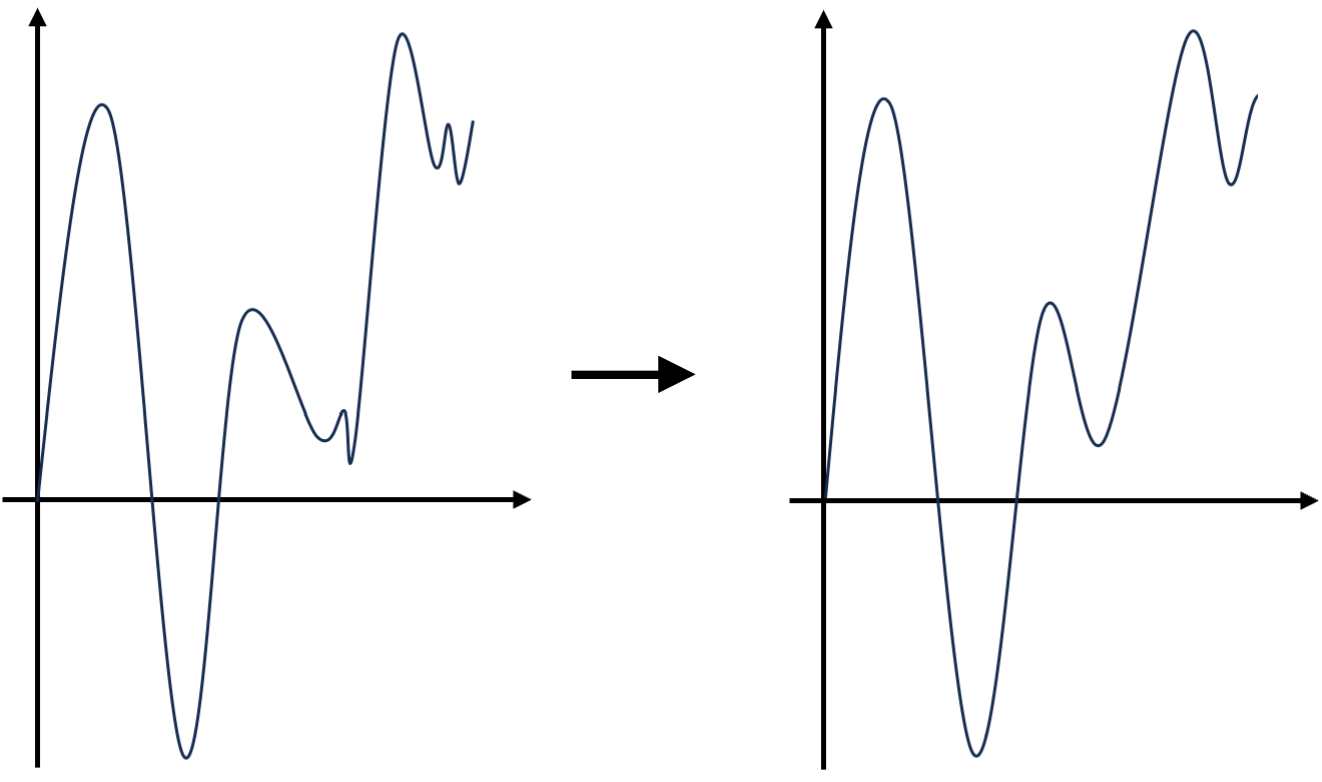
\includegraphics[width=2.5cm]{images/intro/objective_corr.png}};		
					\end{tikzpicture}
				}%
			\end{figure}
		\end{tcolorbox}
	\end{center}

    \textbf{Evolution :}

    \small
    % \setstretch{0.5}
    \begin{itemize}
        \item Geometry : 2D, simple, fixed (as circle, ellipse..) $ \; \rightarrow \;$ 3D / complex / variable
        \item PDE : simple, static (Poisson problem) $\; \rightarrow \;$ complex / dynamic (elasticity, hyper-elasticity)
        \item Neural Network : simple and defined everywhere (PINNs) $\; \rightarrow \;$ Neural Operator
    \end{itemize}
\end{frame}

\begin{frame}{Problem considered}
    \textbf{Elliptic problem with Dirichlet conditions :} \\
    Find $u : \Omega \rightarrow \mathbb{R}^d (d=1,2,3)$ such that
    \begin{equation}
    	\left\{\begin{aligned}
    		&L(u)=-\nabla \cdot (A(x) \nabla u(x)) + c(x)u(x) = f(x) \quad \text{in } \Omega, \\
    		&u(x) = g(x) \quad \text{on } \partial \Omega
    	\end{aligned}\right. \label{edp}
    \end{equation}
	with $A$ a definite positive coercivity condition and $c$ a scalar. We consider $\Delta$ the Laplace operator, $\Omega$ a smooth bounded open set and $\Gamma$ its boundary. 
    
    \textbf{Weak formulation :}
    \begin{equation*}
    	\text{Find } u\in V \text{ such that } a(u, v) = l (v) \forall v\in V
    \end{equation*}
    
    with
    \begin{align*}
    	a(u,v)&=\int_{\Omega} (A(x)\nabla u(x)) \cdot \nabla v(x) + c(x)u(x)v(x) \, dx \\
    	l(v)&=\int_{\Omega} f(x)v(x) \, dx
    \end{align*}
    
    \footnotesize
    \textit{Remark :} For simplicity, we will not consider 1st order terms. 

%    We will define by
%    \begin{equation*}
%        ||u_{ex}-u_{method}||_{0,\Omega}^{(rel)}=\frac{\int_\Omega (u_{ex}-u_{method})^2}{\int_\Omega u_{ex}^2}
%    \end{equation*}
%    the relative error between
%    \begin{itemize}
%        \item $u_{ex}$ : the exact solution  
%        \item $u_{method}$ : the solution obtained by a method \\
%        (can be : FEM or $\phi$-FEM, a correction solver or the prediction of an neural network).
%    \end{itemize}
\end{frame}

\begin{frame}{Numerical methods}
	\textbf{Objective :} Show that the philosophy behind most ofd the methods are the same.
	\begin{center}
		Mesh-based methods \hspace{5pt} // \hspace{5pt} Physically informed learning
	\end{center}
	
	\textbf{Numerical methods :} Discrete an infinite-dimensional problem (unknown = function) and solve it in a finite-dimensional space (unknown = vector).
	\begin{enumerate}[\textbullet]
		\item \textbf{Encoding :} we encode the problem in a finite-dimensional space
		\item \textbf{Approximation :} solve the problem in finite-dimensional space
		\item \textbf{Decoding :} bring the solution back into infinite dimensional space
	\end{enumerate}
	
	\begin{center}
		\begin{tabular}{|c|c|c|}
			\hline
			\textbf{Encoding} & \textbf{Approximation} & \textbf{Decoding} \\
			\hline
			$f \; \rightarrow \theta_f$ & $\theta_f \; \rightarrow \theta_u$ & $\theta_u \; \rightarrow u_\theta$ \\
			\hline
		\end{tabular}
	\end{center}
\end{frame}

	
	\section{Mesh-based methods}
	\subsection{Encoding/Decoding}

\begin{frame}{Encoding/Decoding - FEMs}
	\begin{itemize}[\textbullet]
		\item \textbf{Decoding :} Linear combination of piecewise polynomial function $\varphi_i$.
		\begin{equation*}
			\mathcal{D}_{\theta_u}(x) = \sum_{i=1}^{N}(\theta_u)_i\varphi_i
		\end{equation*}
		$\Rightarrow$ linear decoding $\Rightarrow$ approximation space $V_N$ = vectorial space \\
		$\Rightarrow$ existence and uniqueness of the orthogonal projector
		\item \textbf{Encoding :} Orthogonal projection on vector space $V_N=Vect\{\varphi_1,\dots,\varphi_N\}$.
		\begin{equation*}
			\theta_f=E(f)=M^{-1}b(f)
		\end{equation*}
		with $M_{ij}=\int_\Omega \varphi_i(x)\varphi_j(x)$ and $b_i(f)=\int_\Omega \varphi_i(x)f(x)$. \refappendix{frame:encoding_fems} 
	\end{itemize}
\end{frame}

\subsection{Approximation}

\begin{frame}{Approximation}
	\textbf{Idea :} Project a certain form of the equation onto the vector space $V_N$. \\
	We introduce the residual of the equation defined by
	\begin{equation*}
		R(v) = R_{in}(v)\mathds{1}_{\Omega} + R_{bc}(v)\mathds{1}_{\partial \Omega}
	\end{equation*}
	with 
	\begin{equation*}
		R_{in}(v)=L(v) - f \qquad \text{and} \qquad R_{bc}(v)=v-g
	\end{equation*}
	which respectively define the residues inside $\Omega$ and on the boundary $\partial\Omega$. 
	
	\vspace{10pt}
	
	\textbf{Discretization :} Degrees of freedom problem (which also has a unique solution)
	\begin{center}
		$u=\arg\min_{v\in V_N} J(v) \quad \longrightarrow \quad \theta_u=\arg\min_{\theta\in \mathbb{R}^N} J(\theta) $
	\end{center}
	with $J$ a functional to minimize.
	
	\vspace{10pt}
	
	\textbf{Variants :} Depends on the problem form used for projection.
	
	\begin{center}
		\begin{tabular}{c|c}
			Problem - Energetic form & Problem - Least-square form \\
			Galerkin projection & Galerkin Least-square projection
		\end{tabular}
	\end{center}
\end{frame}

\begin{frame}{Energetic form}
	\textbf{Minimization Problem :}
	\begin{equation}
		u_\theta(x)=\arg\min_{v\in V_N} J(v), \qquad J(v)=J_{in}(v)+J_{bc}(v)\label{minpb_galerkin}
	\end{equation}
	with 
	\begin{equation*}
		J_{in}(v)=\frac{1}{2}\int_\Omega L(v)v - \int_\Omega fv  \qquad \text{et} \qquad J_{bc}(v)=\frac{1}{2}\int_\Omega R_{bc}(v)^2
	\end{equation*}

	\footnotesize	
	\textit{Remark :} This form of the problem is due to the Lax-Milgram theorem as $a$ is symmetrical.
	\normalsize
	
	\footnotesize
	\begin{center}
		\begin{tcolorbox}[
			colback=white, % Couleur de fond de la boîte
			colframe=other, % Couleur du cadre de la boîte
			arc=2mm, % Rayon de l'arrondi des coins
			boxrule=0.5pt, % Épaisseur du cadre de la boîte
			breakable, enhanced jigsaw,
			width=0.8\linewidth
			]
			
			\textbf{Minimization Problem \eqref{minpb_galerkin} $\Leftrightarrow$ PDE \eqref{edp} :}
			
			\centering
			$\nabla_v \; J(v)=R(v) \qquad $ \refappendix{frame:minpb_galerkin} 
			
			\vspace{5pt}
			
			\begin{minipage}{0.1\linewidth}
				\centering
				$u_\theta$ sol \\
				of \eqref{minpb_galerkin}
			\end{minipage} $\Leftrightarrow \; \nabla_{u_\theta} \; J(u_\theta)=0 \; \Leftrightarrow \; \left\{\begin{aligned}
				&R_{in}(u_\theta)=0 \; \text{in} \; \Omega \\
				&u_\theta=g \; \text{on} \; \partial\Omega
			\end{aligned}\right. \; \Leftrightarrow$ \begin{minipage}{0.1\linewidth}
				\centering
				$u_\theta$ sol \\
				of \eqref{edp}
			\end{minipage}
		
			\vspace{5pt}
			
			\begin{minipage}{0.1\linewidth}
				\centering
				\textbf{Min pb}
			\end{minipage} \; \hspace{150pt} \; \begin{minipage}{0.1\linewidth}
				\centering
				\textbf{PDE}
			\end{minipage}
		\end{tcolorbox}
	\end{center}
\end{frame}

\begin{frame}{Galerkin Projection}
	\textbf{Discrete minimization Problem :}
	\begin{equation}
		\theta_u=\arg\min_{\theta\in\mathbb{R}^N} J(\theta), \qquad J(\theta)=J_{in}(\theta)=\frac{1}{2}\int_\Omega L(u_\theta)v_\theta - \int_\Omega fv_\theta \label{minpb_galerkin_discret}
	\end{equation}
%	with 
%	\begin{equation*}
%		
%	\end{equation*}
	
	\footnotesize	
	\textit{Remark :} In practice, boundary conditions can be imposed in different ways. We are therefore only interested in the minimization problem in $\Omega$.
	
	\normalsize	
	
	\textbf{Galerkin projection :} Consists in resolving
	\begin{equation}
		\langle R_{in}(u_\theta(x)),\varphi_i\rangle_{L^2}=0, \qquad \forall i\in\{1,\dots,N\}\label{galerkin_proj}
	\end{equation}

	\footnotesize
	\begin{center}
		\begin{tcolorbox}[
			colback=white, % Couleur de fond de la boîte
			colframe=other, % Couleur du cadre de la boîte
			arc=2mm, % Rayon de l'arrondi des coins
			boxrule=0.5pt, % Épaisseur du cadre de la boîte
			breakable, enhanced jigsaw,
			width=\linewidth
			]
			
			\textbf{Galerkin Projection \eqref{galerkin_proj} $\Leftrightarrow$ PDE \eqref{edp} :}
			
			\centering
			$\nabla_\theta \; J(\theta)=\left(\int_\Omega R_{in}(v_\theta)\varphi_i\right)_{i=1,\dots,N} \qquad $ \refappendix{frame:galerkin_proj} 
			
			\vspace{5pt}
			
			\begin{minipage}{0.1\linewidth}
				\centering
				$u_\theta$ sol \\
				of \eqref{edp}
			\end{minipage} $\; \Leftrightarrow \;$	\begin{minipage}{0.1\linewidth}
				\centering
				$u_\theta$ sol \\
				of \eqref{minpb_galerkin}
			\end{minipage} $\; \Leftrightarrow \;$	\begin{minipage}{0.1\linewidth}
				\centering
				$u_\theta$ sol \\
				of \eqref{minpb_galerkin_discret}
			\end{minipage} $\Leftrightarrow \; \nabla_\theta \; J(\theta)=0 \; \Leftrightarrow$ \begin{minipage}{0.1\linewidth}
				\centering
				$u_\theta$ sol \\
				of \eqref{galerkin_proj}
			\end{minipage}
		
			\vspace{5pt}
		
			\begin{minipage}{0.1\linewidth}
				\centering
				\textbf{PDE}
			\end{minipage} $\; \quad \;$ \begin{minipage}{0.1\linewidth}
				\centering
				\textbf{Min pb}
			\end{minipage} $\; \quad \;$ \begin{minipage}{0.1\linewidth}
				\centering
				\textbf{Discrete} \\
				\textbf{min pb}
			\end{minipage} \; \hspace{60pt} \; \begin{minipage}{0.1\linewidth}
				\centering
				\textbf{Galerkin} \\
				\textbf{projection}
			\end{minipage}
		\end{tcolorbox}
	\end{center}
\end{frame}

\begin{frame}{Least-Square form}
	\textbf{Minimization Problem :}
	\begin{equation}
		u_\theta(x)=\arg\min_{v\in V_N} J(v), \qquad J(v)=J_{in}(v)+J_{bc}(v)\label{minpb_leastsquare}
	\end{equation}
	with 
	\begin{equation*}
		J_{in}(v)=\frac{1}{2}\int_\Omega R_{in}(v)^2  \qquad \text{and} \qquad J_{bc}(v)=\frac{1}{2}\int_\Omega R_{bc}(v)^2
	\end{equation*}
	
	\footnotesize	
	\textit{Remark :} This form of the problem is due to the Lax-Milgram theorem as $a$ is symmetrical.
	\normalsize
	
	\footnotesize
	\begin{center}
		\begin{tcolorbox}[
			colback=white, % Couleur de fond de la boîte
			colframe=other, % Couleur du cadre de la boîte
			arc=2mm, % Rayon de l'arrondi des coins
			boxrule=0.5pt, % Épaisseur du cadre de la boîte
			breakable, enhanced jigsaw,
			width=\linewidth
			]
			
			\textbf{Minimization Problem \eqref{minpb_leastsquare} $\Leftrightarrow$ PDE \eqref{edp} :}
			
			\centering
			$\nabla_v \; J(v)=L(R(v))\mathds{1}_\Omega+(v-g)\mathds{1}_{\partial\Omega} \qquad $ \refappendix{frame:minpb_leastsquare} 
			
			\vspace{5pt}
			
			\begin{minipage}{0.1\linewidth}
				\centering
				$u_\theta$ sol \\
				of \eqref{minpb_leastsquare}
			\end{minipage} $\Leftrightarrow \; \nabla_{u_\theta} \; J(u_\theta)=0 \; \Leftrightarrow \; \left\{\begin{aligned}
				&L(R(u_\theta))=0 \; \text{in} \; \Omega \\
				&R(u_\theta)=0 \; \text{on} \; \partial\Omega
			\end{aligned}\right. \; \Leftrightarrow \; R(u_\theta)=0 \; \Leftrightarrow$ \begin{minipage}{0.1\linewidth}
				\centering
				$u_\theta$ sol \\
				of \eqref{edp}
			\end{minipage}
			
			\vspace{5pt}
			
			\begin{minipage}{0.1\linewidth}
				\centering
				\textbf{Min pb}
			\end{minipage} \; \hspace{210pt} \; \begin{minipage}{0.1\linewidth}
				\centering
				\textbf{PDE}
			\end{minipage}
		\end{tcolorbox}
	
		\hl{A modifier !}
	\end{center}
\end{frame}

\begin{frame}{Least-Square Galerkin Projection}
	\textbf{Discrete minimization Problem :}
	\begin{equation}
		\theta_u=\arg\min_{\theta\in\mathbb{R}^N} J(\theta), \qquad J(\theta)=J_{in}(\theta)=\frac{1}{2}\int_\Omega (L(u_\theta) - f)^2 \label{minpb_leastsquare_discret}
	\end{equation}
	%	with 
	%	\begin{equation*}
		%		
		%	\end{equation*}
	
	\footnotesize	
	\textit{Remark :} In practice, boundary conditions can be imposed in different ways. We are therefore only interested in the minimization problem in $\Omega$.
	
	\normalsize	
	
	\textbf{Galerkin projection :} Consists in resolving
	\begin{equation}
		\langle R_{in}(u_\theta(x)),(\nabla_\theta R_{in}(u_\theta(x)))_i\rangle_{L^2}=0, \qquad \forall i\in\{1,\dots,N\}\label{leastsquare_proj}
	\end{equation}
	
	\footnotesize
	\begin{center}
		\begin{tcolorbox}[
			colback=white, % Couleur de fond de la boîte
			colframe=other, % Couleur du cadre de la boîte
			arc=2mm, % Rayon de l'arrondi des coins
			boxrule=0.5pt, % Épaisseur du cadre de la boîte
			breakable, enhanced jigsaw,
			width=\linewidth
			]
			
			\textbf{Least-Square Galerkin Projection \eqref{leastsquare_proj} $\Leftrightarrow$ PDE \eqref{edp} :}
			
			\centering
			$\nabla_\theta \; J(\theta)=\left(\int_\Omega L(R_{in}(v_\theta))\varphi_i\right)_{i=1,\dots,N} \qquad $ \refappendix{frame:leastsquare_proj} 
			
			\vspace{5pt}
			
			\begin{minipage}{0.1\linewidth}
				\centering
				$u_\theta$ sol \\
				of \eqref{edp}
			\end{minipage} $\; \Leftrightarrow \;$	\begin{minipage}{0.1\linewidth}
				\centering
				$u_\theta$ sol \\
				of \eqref{minpb_leastsquare}
			\end{minipage} $\; \Leftrightarrow \;$	\begin{minipage}{0.1\linewidth}
				\centering
				$u_\theta$ sol \\
				of \eqref{minpb_leastsquare_discret}
			\end{minipage} $\Leftrightarrow \; \nabla_\theta \; J(\theta)=0 \; \Leftrightarrow$ \begin{minipage}{0.1\linewidth}
				\centering
				$u_\theta$ sol \\
				of \eqref{leastsquare_proj}
			\end{minipage}
			
			\vspace{5pt}
			
			\begin{minipage}{0.1\linewidth}
				\centering
				\textbf{PDE}
			\end{minipage} $\; \quad \;$ \begin{minipage}{0.1\linewidth}
				\centering
				\textbf{Min pb}
			\end{minipage} $\; \quad \;$ \begin{minipage}{0.1\linewidth}
				\centering
				\textbf{Discrete} \\
				\textbf{min pb}
			\end{minipage} \; \hspace{60pt} \; \begin{minipage}{0.15\linewidth}
				\centering
				\textbf{LS Galerkin} \\
				\textbf{projection}
			\end{minipage}
		\end{tcolorbox}
	\end{center}
\end{frame}

\begin{frame}{Steps Decomposition - FEMs}
	\begin{center}
		\renewcommand{\arraystretch}{1.5}
		\begin{tabular}{|c|c|c|c|}
			\hline
			\textbf{Encoding} & \multicolumn{2}{c|}{\textbf{Approximation}} & \textbf{Decoding} \\
			\hline
			$f \; \rightarrow \theta_f$ & \multicolumn{2}{c|}{$\theta_f \; \rightarrow \theta_u$} & $\theta_u \; \rightarrow u_\theta$ \\
			\hline
			\multirow{3}{*}{$\begin{aligned}
				\theta_f&=\mathcal{E}(f) \\
				&=M^{-1}b(f)
			\end{aligned}$} & Galerkin & LS Galerkin & \multirow{3}{*}{$\begin{aligned}
				u_\theta(x)&=\mathcal{D}_\theta(x) \\
				&=\sum_{i=1}^N (\theta_u)_i\varphi_i
			\end{aligned}$} \\
			 & \small $\langle R(u_\theta),\varphi_i\rangle_{L^2}=0$ & \small $\langle R(u_\theta),(\nabla_\theta R(u_\theta))_i\rangle_{L^2}=0$ & \\
			\cline{2-3}
			 & \multicolumn{2}{c|}{$A\theta_u=B$} & \\
			 \hline
		\end{tabular}
	\end{center}

	\footnotesize
	\textit{\textbf{Example :}} Galerkin projection.
	
	\begin{minipage}{0.48\linewidth}
		For $i\in\{1,\dots,N\}$,
		\begin{align*}
			\langle R(u_\theta),\varphi_i\rangle_{L^2}&=0 \\
			\iff \quad \int_\Omega L(u_\theta)\varphi_i &= \int_\Omega f\varphi_i \\
			\iff \quad \sum_{j=1}^N(\theta_u)_j \int_\Omega \varphi_i L(\varphi_j) &= \int_\Omega f\varphi_i
		\end{align*}
	\end{minipage}
	\begin{minipage}{0.48\linewidth}
		\begin{equation*}
			A\theta_u=B \; \text{with}
		\end{equation*}
		\begin{equation*}
			A_{i,j} = \int_\Omega \varphi_i L(\varphi_j) \quad \text{,} \quad B_i =  \int_\Omega f\varphi_i
		\end{equation*}
	\end{minipage}
\end{frame}
	
	\section{Physically Informed Learning}
	\begin{frame}{Neural Network considered}
    \vspace{-2pt}
    We consider a parametric NN with 4 inputs and 4 outputs, defined by
    $$U_\theta(\bm{x},\bm{\mu}) = \big(u_{1,\theta},u_{2,\theta},p_\theta,T_\theta)(\bm{x},\bm{\mu}).$$
    
    The Dirichlet boundary conditions are imposed on the outputs of the MLP by a \textbf{post-processing} step. \citep{Sukumar_2022}
    
    \begin{center}
        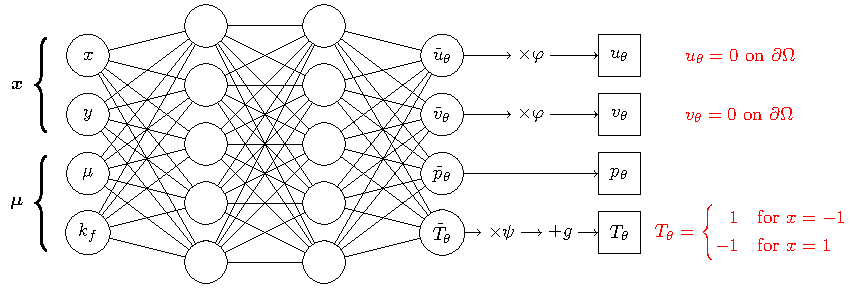
\includegraphics[width=0.85\linewidth]{images/pinn/network/network.pdf}
    \end{center}

    \vspace{-5pt}
    We consider two levelsets functions $\varphi_1$ and $\varphi_2$, and the linear function $g$ defined by
    \begin{equation*}
        \varphi_1(x,y) = (x-1)(x+1)(y-1)(y+1),
    \end{equation*}
    \begin{equation*}
        \varphi_2(x,y) = (x-1)(x+1) \quad \text{and} \quad g(x,y) = 1 - (x+1).
    \end{equation*}
\end{frame}

\begin{frame}{PINN training}
    \vspace{-4pt}
    \textbf{Approximate the solution of \eqref{eq:Pb} by a PINN :} Find the optimal weights $\theta^\star$, such that
	
    \vspace{-8pt}
    \begin{equation}
		\label{eq:opt_pb}
		\theta^\star = \argmin_{\theta}	\big( \; \textcolor{orange}{J_{inc}(\theta)} + \textcolor{orange}{J_{mom}(\theta)} + \textcolor{orange}{J_{ener}(\theta)} + \textcolor{darkred}{J_{ad}(\theta)} \; \big),
		\tag{$\mathcal{P}_\theta$}
	\end{equation}

    \vspace{-2pt}
	where the different cost functions\footnote[frame,1]{Discretized by a random process using Monte-Carlo method.} are defined by
	\vspace{5pt}

	\begin{minipage}{0.24\linewidth}
		\centering
		\textcolor{darkred}{adiabatic condition}
        
		\vspace{12pt}
		\textcolor{orange}{$3$ residual losses}
	\end{minipage}
	\begin{minipage}{0.68\linewidth}
		\centering
        \fcolorbox{darkred}{white}{
            $J_{ad}(\theta) =
            \int_{\mathcal{M}}\int_{\Gamma_\text{ad}} \big| \frac{\partial T_\theta(\bm{x},\bm{\mu})}{\partial n} \big|^2 d\bm{x} d\bm{\mu},$}
        
        \vspace{3pt}
		\fcolorbox{orange}{white}{
            $J_{\textbullet}(\theta) =
                \int_{\mathcal{M}}\int_{\Omega}
                \big| R_{\textbullet}(U_\theta(\bm{x},\bm{\mu});\bm{x},\bm{\mu}) \big|^2 d\bm{x} d\bm{\mu},$}
	\end{minipage}
    
    \vspace{5pt}
    with $U_\theta$ the parametric NN and $\textbullet$ the PDE considered (i.e. $inc$, $mom$ or $ener$).

    %\footnote[frame,2]{We consider a MLP with 5 hidden layers ($40,60,60,60,40$) and a 'sine' activation function. We train the PINN over $10000$ epochs ($3000$ ADAM / $7000$ LBFGS) with $40000$ collocation points in $\Omega$ and $30000$ points on the boundary $\partial\Omega\vert_{y=\pm 1}$.}
    
    \vspace{-7pt}
    \vspace{3pt}    
    \begin{center}
        \begin{minipage}{0.62\linewidth}
            \centering
            \vspace{-8pt}
            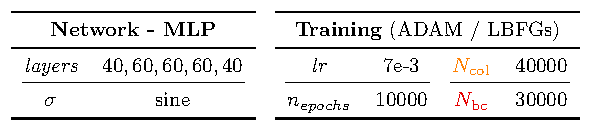
\includegraphics[width=0.94\linewidth]{images/pinn/training_param/training_param.pdf}
        \end{minipage}
        \begin{minipage}{0.36\linewidth}
            \centering
            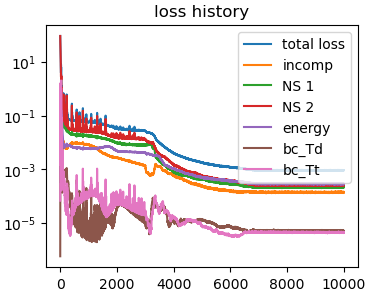
\includegraphics[width=0.84\linewidth]{images/pinn/training/test4_v5.png}
        \end{minipage}
    \end{center}
    
    \vspace{-8pt}
\end{frame}

\begin{frame}{Prediction on $\bm{\mu}^{(1)} = (0.1,0.1)$}
    \vspace{-4pt}
    \textbf{Prediction :} \begin{minipage}{0.26\linewidth}
        \centering
        $u_{1,\theta}$ \\
        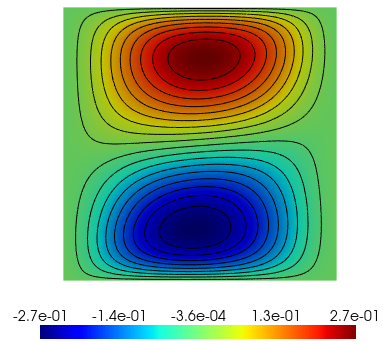
\includegraphics[width=0.95\linewidth]{images/pinn/training/PINN_plot_case4_v2_param1_u1.png}
    \end{minipage} \; \begin{minipage}{0.26\linewidth}
        \centering
        $u_{2,\theta}$ \\
        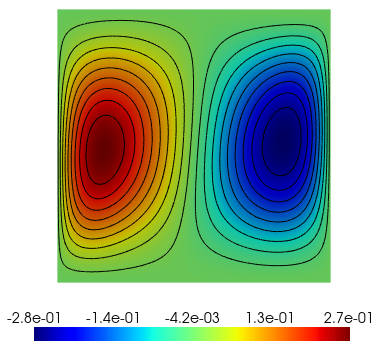
\includegraphics[width=0.95\linewidth]{images/pinn/training/PINN_plot_case4_v2_param1_u2.png}
    \end{minipage} \; \begin{minipage}{0.26\linewidth}
        \centering
        $T_\theta$ \\
        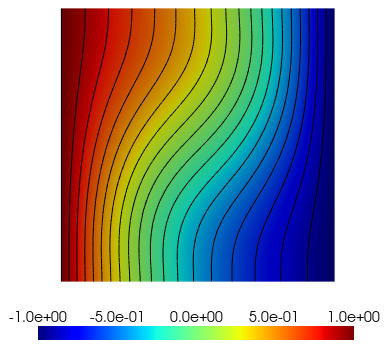
\includegraphics[width=0.95\linewidth]{images/pinn/training/PINN_plot_case4_v2_param1_T.png}
    \end{minipage}

    \vspace{8pt}

    \textbf{Error map :} \begin{minipage}{0.26\linewidth}
        \centering
        $u_{1,\text{ref}}-u_{1,\theta}$ \\
        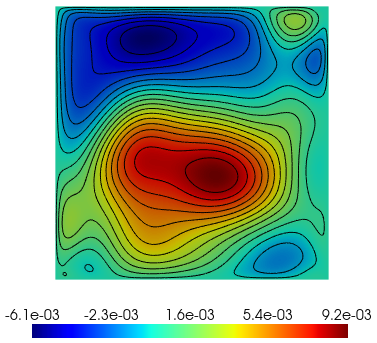
\includegraphics[width=0.95\linewidth]{images/pinn/training/PINN_error_plot_case4_v2_param1_u1.png}
    \end{minipage} \; \begin{minipage}{0.26\linewidth}
        \centering
        $u_{2,\text{ref}}-u_{2,\theta}$ \\
        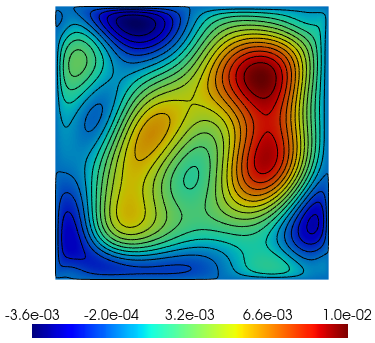
\includegraphics[width=0.95\linewidth]{images/pinn/training/PINN_error_plot_case4_v2_param1_u2.png}
    \end{minipage} \; \begin{minipage}{0.26\linewidth}
        \centering
        $T_\text{ref}-T_\theta$ \\
        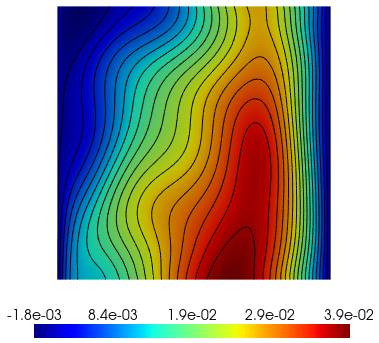
\includegraphics[width=0.95\linewidth]{images/pinn/training/PINN_error_plot_case4_v2_param1_T.png}
    \end{minipage}

    \vspace{8pt}

    \textbf{$L^2$ error :} \hspace{25pt} $2.98\times10^{-2} \hspace{42pt} 3.17\times10^{-2} \hspace{42pt}  3.90\times10^{-2}$

    \vspace{-2pt}
    \textbf{\small (relative)}
\end{frame}
	
	\section{Our hybrid method}
	\begin{frame}{$\phi$-FEM Method}
	\textbf{Main ideas :} \small
	
	\begin{minipage}[t]{0.48\linewidth}
		\begin{itemize}[\textbullet]
			\item Domain defined by a LevelSet Function $\phi$.
		\end{itemize}
		\centering
		\pgfimage[width=0.6\linewidth]{images/hybrid/PhiFEM_level_set.png}
	\end{minipage} \hfill
	\begin{minipage}[t]{0.48\linewidth}
		\begin{itemize}[\textbullet]
			\item We are looking for $w$ such that $u=\phi w+g$. \\
			Thus, the decoder is written as
			\begin{equation*}
				u_\theta(x)=\mathcal{D}_{\theta_w}(x) = \phi(x)\sum_{i=1}^{N}(\theta_w)_i\varphi_i+g(x)
			\end{equation*}
		\end{itemize}
	\end{minipage}

	\begin{itemize}[\textbullet]
		\item Mesh of a fictitious domain containing $\Omega$.
	\end{itemize}
	\begin{center}
		\begin{minipage}{0.43\linewidth}
			\centering
			\pgfimage[width=\linewidth]{images/more/PhiFEM_domain.png}
		\end{minipage} \hfill
		\begin{minipage}{0.1\linewidth}
			\centering
			\pgfimage[width=\linewidth]{images/more/PhiFEM_fleche.png} 
		\end{minipage} \hfill
		\begin{minipage}{0.43\linewidth}
			\centering
			\pgfimage[width=\linewidth]{images/more/PhiFEM_domain_considered.png}
		\end{minipage}
	\end{center}
\end{frame}

\begin{frame}{Impose exact BC in PINNs}
	\hl{A compléter !}
\end{frame}

\begin{frame}{Correct PINNs prediction with $\phi$FEM}
	\hl{A compléter !}
\end{frame}
	
	\section{Conclusion} %perspectives
	
	\begin{frame}{Conclusion - What has been seen }
		\begin{itemize}[\textbullet]
			\item "Physical Informed Learning" methods are simply an extension of classic numerical methods such as FEM, where the decoder belongs to a variety (whose properties are different from those of vector spaces).
			\item These approaches have real advantages in high dimensions, particularly in the context of parametric PDEs.
			\item Moreover, as they are mesh-free methods, they have a major advantage in the context of complex geometries.
		\end{itemize}
	\end{frame}

	\begin{frame}[label={lastslide}]{Conclusion - Our hybrid approach}
		\textbf{Interest of our approach:} 
		\begin{itemize}[\textbullet]
			\item It combines
			\begin{itemize}[\ding{217}]
				\item Speed of neural networks in predicting a solution
				\item Precision of FEM methods to correct and certify the prediction of the neural network (which can be completely wrong, on an unknown dataset for example)
			\end{itemize}
			\item In the context of complex geometry (or in application domains such as real-time or shape optimisation), like NNs, $\phi$-FEM makes it possible to avoid mesh (re-)generation.
		\end{itemize}
		
		\textbf{Current results:}
		\begin{itemize}[\textbullet]
			\item Encouraging results on simple geometries \refappendix{frame:results}
			\item Difficulties on complex geometries - Importance of the regularity of the LevelSet function \\
			$\rightarrow$ Next step: learning levelset functions (Eikonal equation)
		\end{itemize}
	\end{frame}

	\begin{frame}
		\vfill
		\centering
		\LARGE Thank you !
		\vfill
	\end{frame}
	
%	\section{Bibliography}
	
	{\setbeamertemplate{footline}{} 
		\begin{frame}{Bibliography}
			\small
			% \vspace{30pt}
			% \setstretch{0.2}
			% \AtNextBibliography{\small}
			\printbibliography[heading=none]
		\end{frame}
	}
	\addtocounter{framenumber}{-1} 
	
	\appendix
	
	\begin{frame}{\appendixname~\insertframenumber~: Encoding - FEMs}\phantomsection\label{frame:encoding_fems}
	
	Pourquoi ?
\end{frame}

%\begin{frame}{Architecture of the FNO}
%    \begin{center}
%        \centering
%        \pgfimage[width=\linewidth]{images/more/FNO/FNO_schema.png}
%    \end{center}
%    \textbf{Input $X$} of shape (bs,ni,nj,nk) \qquad \qquad \textbf{Output $Y$} of shape (bs,ni,nj,1) \\
%    with bs the batch size, ni and nj the grid resolution and nk the number of channels.
%\end{frame}
%
%\begin{frame}{Description of the FNO architecture}
%    \begin{center}
%        \centering
%        \pgfimage[width=\linewidth]{images/more/FNO/FNO_schema_moitie1.png}
%    \end{center}
%    \begin{enumerate}[\ding{217}]
%        \item perform a $P$ transformation, to move to a space with more channels (to build a sufficiently rich representation of the data)
%        \item apply $L$ Fourier layers defined by
%        $$\mathcal{H}_\theta^l(\tilde{X})=\sigma\left(\mathcal{C}_\theta^l(\tilde{X})+\mathcal{B}_\theta^l(\tilde{X})\right),\; l=1,\dots,L$$
%        with $\tilde{X}$ the input of the current layer and
%        \begin{itemize}
%            \item $\sigma$ an activation function (ReLU or GELU)
%            \item $\mathcal{C}_\theta^l$ : convolution sublayer (convolution performed by Fast Fourier Transform)
%            \item $\mathcal{B}_\theta^l$ : "bias-sublayer"
%        \end{itemize}
%        \item return to the target dimension by performing a $Q$ transformation (in our case, the number of output channels is 1)
%    \end{enumerate}
%\end{frame}
%
%\begin{frame}{Fourier Layer Structure}
%    \setstretch{0.5}
%    \textbf{Convolution sublayer : } \quad $\mathcal{C}_\theta^l(X)=\mathcal{F}^{-1}(\mathcal{F}(X)\cdot\hat{W})$ \quad
%    \begin{minipage}{0.3\linewidth}
%        \vspace{-15pt}
%        \centering
%        \pgfimage[width=\linewidth]{images/more/FNO/FNO_schema_moitie2.png}
%    \end{minipage}
%    \begin{enumerate}[\ding{217}]
%        \item $\hat{W}$ : a trainable kernel
%        \item $\mathcal{F}$ : 2D Discrete Fourier Transform (DFT) defined by
%        \begin{equation*}
%            \mathcal{F}(X)_{ijk}=\frac{1}{ni}\frac{1}{nj}\sum_{i'=0}^{ni-1}\sum_{j'=0}^{nj-1}X_{i'j'k}e^{-2\sqrt{-1}\pi\left(\frac{ii'}{ni}+\frac{jj'}{nj}\right)}
%        \end{equation*}
%        $\mathcal{F}^{-1}$ : its inverse.
%        \item $(Y\cdot\hat{W})_{ijk}=\sum_{k'}Y_{ijk'}\hat{W}_{ijk'} \quad \Rightarrow \quad$ applied channel by channel
%    \end{enumerate} \; \\
%    \textbf{Bias-sublayer :} \quad  $\mathcal{B}_\theta^l(X)_{ijk}=\sum_{k'}X_{ijk}W_{k'k}+B_k$ \quad
%    \begin{minipage}{0.3\linewidth}
%        \vspace{-10pt}
%        \pgfimage[width=0.3\linewidth]{images/more/FNO/FNO_schema_moitie2_bis.png}
%    \end{minipage}
%    \begin{enumerate}[\ding{217}]
%        \item 2D convolution with a kernel of size 1
%        \item allowing channels to be mixed via a kernel without allowing interaction between pixels.
%    \end{enumerate}
%\end{frame}
%
%\begin{frame}{Dual method -  Poisson Problem}
%    \setstretch{0.5}		
%    \textbf{Problem :} Find $u$ on $\Omega_h$ and $p$ on $\Omega_h^\Gamma$ such that
%    \begin{align*}
%        \int_{\Omega_h}\nabla u\nabla v&-\int_{\partial\Omega_h}\frac{\partial u}{\partial n} v + \frac{\gamma}{h^2} \sum_{T\in\mathcal{T}_h^\Gamma}\int_T \left(u-\frac{1}{h}\phi p\right)\left(v-\frac{1}{h}\phi q\right) \\
%        &+ G_h(u,v) = \int_{\Omega_h}fv + G_h^{rhs}(v), \; \forall v \; \text{on } \Omega_h, \; q \; \text{on } \Omega_h^\Gamma
%    \end{align*}
%    with $\gamma$ an other positive stabilization parameter and $G_h$ and $G_h^{rhs}$ the stabilization terms defined previously.
%    
%    For the non homogeneous case, we replace
%    $$\int_T \left(u-\frac{1}{h}\phi p\right)\left(v-\frac{1}{h}\phi q\right) \quad \rightarrow \quad \int_T\left(u-\frac{1}{h}\phi p-g\right)\left(v-\frac{1}{h}\phi q\right)$$ 
%    by assuming $g$ is defined on $\Omega_h^\Gamma$
%\end{frame}
	
\end{document}
